\begin{figure}
  \centering
  \begin{subfigure}[b]{0.42\textwidth}
    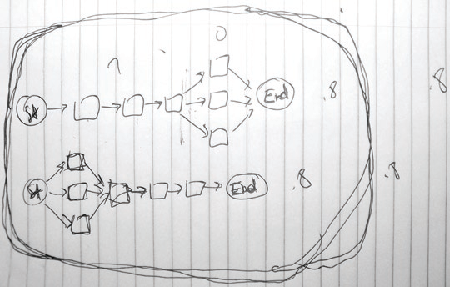
\includegraphics[width=\linewidth]{img/sketch-type-project-management.pdf}
    \caption{Project management diagram showing task precedence of two
      projects. Hastily drawn boxes and arrows represent abstract
      activities.}
    \label{fig:sketch-type-pm}
  \end{subfigure}
  \hspace{1cm}
  \begin{subfigure}[b]{0.42\textwidth}
    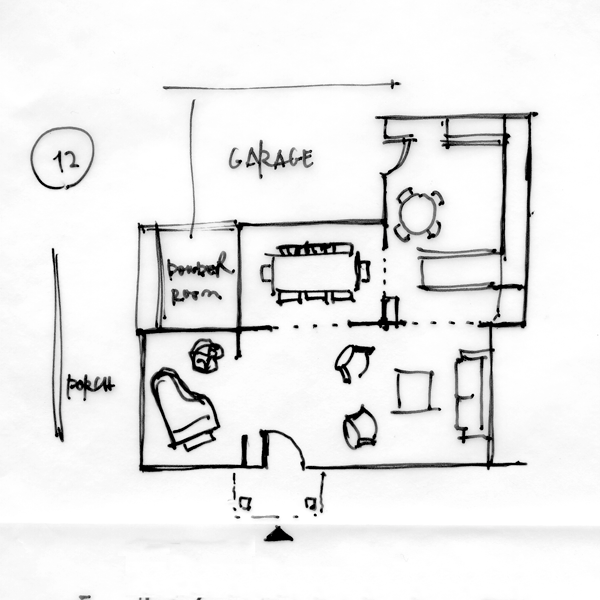
\includegraphics[width=\linewidth]{img/sketch-type-architecture.pdf}
    \caption{An architect's floor plan sketch. It includes text, 
      spatial information, and symbols representing household
      items like a piano or dining table.}
    \label{fig:sketch-type-architecture}
  \end{subfigure}
  
  \caption[Project management and Architecture sketches]{Sketches vary
    in domain and in the visual characteristics of marks.}
  \label{fig:types-of-sketches}

\end{figure}
